
\section*{Conclusiones}

% Este espacio podría estar bueno para enunciar posibles vetas de investigación a partir de lo que paso. Podriamos aclarar que fue un proyecto práctico que detonó reflexiones e ideas que se pueden desarrollar más adelante. Aquí también puede anunciarse el trabajo con three y anti 

% La pregunta principial sería: ¿Se cumplió la hipótesis/premisa del software escrito? 

% Comenté lo de abajo, creo que es redundante

% Los usuarios pudieron compartir una experiencia ligera para el navegador de manera co-presencial, aprovechando las posibilidades de las tecnologías de transmisión de audio y video. Destacamos la importancia de plantear soluciones compartibles en lo que respecta a la transmisión de audio-imagen. La escritura de esta parte de \textit{Panorama} fue utilizado en el marco de otros eventos y ciclos.

%El proyecto no tuvo un plan de acción específico para la realización de mediciones durante los conciertos, a pesar de que el control del servidor lo permitió. Sin embargo, la lectura de información a partir de una simulación del evento arroja datos importantes en este sentido.

%Sobre las impresiones del público, fue posible realizar un cuestionario durante \textit{Pruebas Proféticas}. 

%La importancia de una infraestructura tecnológica y social. Esto se puede entretejer a partir de decisiones curatoriales que vinculan potencial tecnológico con alianzas entre actores. 

%Del lado teórico es necesario convenir y reforzar un corpus de conceptos para la investigación sobre Tecnología Musical. Detección de campos y persectivas de investigación: las agencias que están presentes en eventos que se desenvuelven con tecnología.


%Las consecuencias estéticas, tecnológicas e investigativas de estos eventos apuntan a la necesidad de establecer un corpus de conceptos y perspectivas que posibiliten la observación de nuevas prácticas artísticas con medios \citep{shankenCanon} que implican la interpretación musical digital y que se desborda a otros campos. Esta intención podría incluir la estética de estas prácticas, la programación del software que las posibilita, su condición como software escrito y ejecutado \citep{speakingCode} y las consecuencias sociales y políticas de la distribución en red. % Esto podría estar después 

%Los eventos realizados en la diversidad de plataformas anteriormente descrita han utilizado ligas a internet que de acuerdo a la fecha consultada, redireccionan a distintos espacios virtuales. A diferencia de los sitios que utilizan texto y entornos de programación web como HTML, la mezcla de módulos y el uso de frameworks dedicados que utilizan renderizadores 3d como webGL, motores de audio como Web Audio API o plataformas de transmisión de audio y video personalizadas y efímeras dificultan la documentación convencional. La labor se complica cuando el mantenimiento de estos espacios sobrepasa los alcances temporales o económicos del proyecto. El reto metodológico que esto supone es un asunto pendiente para las investigaciones que hacen referencia a programas de computadora como recurso. En este sentido, la referencia a repositorios de código públicos podrían arrojar soluciones para la documentación y arqueología de los desarrollos tecnológicos. Una alternativa posible es \textit{Wayback Machine}\footnote{``\textit{The Wayback Machine} es una iniciativa de Internet Archive para construir una librería digital de sitios de Internet y otros artefactos culturales en formato digital''. \url{http://web.archive.org/} (Consultado el \today)} y en general, reestructurar la forma en la que se documenta y experimentan los sitios web. 

%Estas perspectivas pueden extenderse hacia una postura para la investigación de tecnología y el papel que juegan en la política de los espacios físicos y virtuales, como el cuarto propio \citep{cuartopropio} o el buen conocer \citep{plato}. Podríamos relacionar estos procesos con el giro de los nuevos medios descrito por \cite{manovichlanguage}, las implicaciones sociales de este giro y sobre todo, las consecuencias estéticas que a partir de este se abren y desenvuelven en el performance musical por medio de la computadora y otras prácticas afines. 

%Destacamos el giro de los nuevos medios como un cambio de paradigma que la tecnología musical debe considerar por las implicaciones de los usos/críticas de las tecnologías de la información, las tendencias para la resolución de problemas relacionados con gestión de datos y las consecuencias estéticas que a veces se empalman y otras rebasan a la música y las perspectivas de investigación asociadas a esta disciplina. El rodeo o la realización de un motivo tecnológico como una perspectiva de investigación que pueda aportar en el aspecto tecnológico y teórico-metodológico, sobre todo en campos que lo permiten como humanidades, artes y específicamente, investigación que implica música y expresiones audiovisuales con tecnología.

%\color{Fuchsia}

%A manera de cierre, consideramos que la observación y la investigación podría extenderse a manifiestos, posturas políticas y alternativas en la organización que dialogan con la escritura de software como desarrollo tecnológico y como acto creativo. Tal es el caso de la práctica de \textit{live coding} y la transparencia de los procesos o el uso de interfaces de texto \citep{collinsLivecoding}, el manifiesto de una servidora feminista \citep{feministserver} o la arquitectura de distribución de información par a par\footnote{\textit{P2P} (par a par) por sus siglas en inglés.  ``La arquitectura de una red distribuida puede ser llamada Par a Par (P-to-P, P2P, ...)   si los participantes comparten una parte de los recursos de su propio software (poder de procesamiento, capacidad de almacenamiento, capacidad de conexión a la red, impresoras,...) Estos recursos compartidos son necesarios para proveer el Servicio y el contenido ofrecido por la red... Estos son accedidos por otros pares directamente sin pasar por entidades intermediarias." \citep{p2p}} que persigue la distribución y la descentralización en redes que posibilitan espacios virtuales \citep{cyberspace} y que incluso puede extenderse al autocuidado y formas alternativas de expresar relaciones sociales en red \citep{dwc} o desmantelar y reconfigurar tecnologías en relación a la estética, a la tecnología y a la organización social distribuida. 


El navegador, como una tecnología accesible en términos de recursos de la computadora y de dispositivos o instalaciones adicionales, permitió la escritura de espacios inmersivos con \textit{Panorama}. Consideramos que la optimización de estos espacios para dispositivos móviles y la exploración extendida para la transmisión de datos bajo la lógica de la compartición par a par\footnote{\textit{P2P} (par a par) por sus siglas en inglés.  ``La arquitectura de una red distribuida puede ser llamada Par a Par (P-to-P, P2P, ...)  si los participantes comparten una parte de los recursos de su propio software (poder de procesamiento, capacidad de almacenamiento, capacidad de conexión a la red, impresoras,...) Estos recursos compartidos son necesarios para proveer el Servicio y el contenido ofrecido por la red... Estos son accedidos por otros pares directamente sin pasar por entidades intermediarias." \citep{p2p}} son puntos que quedan pendientes para la escritura e investigación futuras. 

A diferencia de los sitios que utilizan texto y entornos de programación web como HTML, la mezcla de módulos y el uso de frameworks dedicados que utilizan renderizadores 3d como webGL, motores de audio como Web Audio API o plataformas de transmisión de audio y video personalizadas y efímeras dificultan la documentación convencional. La labor se complica cuando el mantenimiento de estos espacios sobrepasa los alcances temporales o económicos del proyecto. El reto metodológico que esto supone es un asunto pendiente para las investigaciones que hacen referencia a programas de computadora como recurso de investigación. En este sentido, la referencia a repositorios de código públicos podrían arrojar soluciones para la documentación y arqueología de los desarrollos tecnológicos. Una alternativa posible es \textit{Wayback Machine}\footnote{``\textit{The Wayback Machine} es una iniciativa de Internet Archive para construir una librería digital de sitios de Internet y otros artefactos culturales en formato digital''. \url{http://web.archive.org/} (Consultado el \today)} y en general, reestructurar la forma en la que se documenta y experimenta la web. 


El trayecto de investigación involucrado en \textit{Panorama} arrojó motivaciones para la realización de piezas que se ejecuten entre espacio, tiempo e interpretación. Al momento de escritura hay dos proyectos que atienden estos aspectos y que pueden extender la discusión: THREE.studies\footnote{Versión fija en la web y repositorio: \url{http://threecln.piranhalab.cc/} \url{https://github.com/EmilioOcelotl/THREE.studies}} y anti (Figura \ref{fig:anti}).\footnote{Versión web en construcción. Repositorio: \url{https://github.com/EmilioOcelotl/anti}} Teniendo en cuenta la extensión de la realización estética y tecnológica, una posible agenda de creación investigación podría tener en cuenta la colaboración y la realización de piezas en un contexto post-pandemia que podría acoplar aspectos de la co-presencia física y de la interacción digital. 

\begin{figure}
  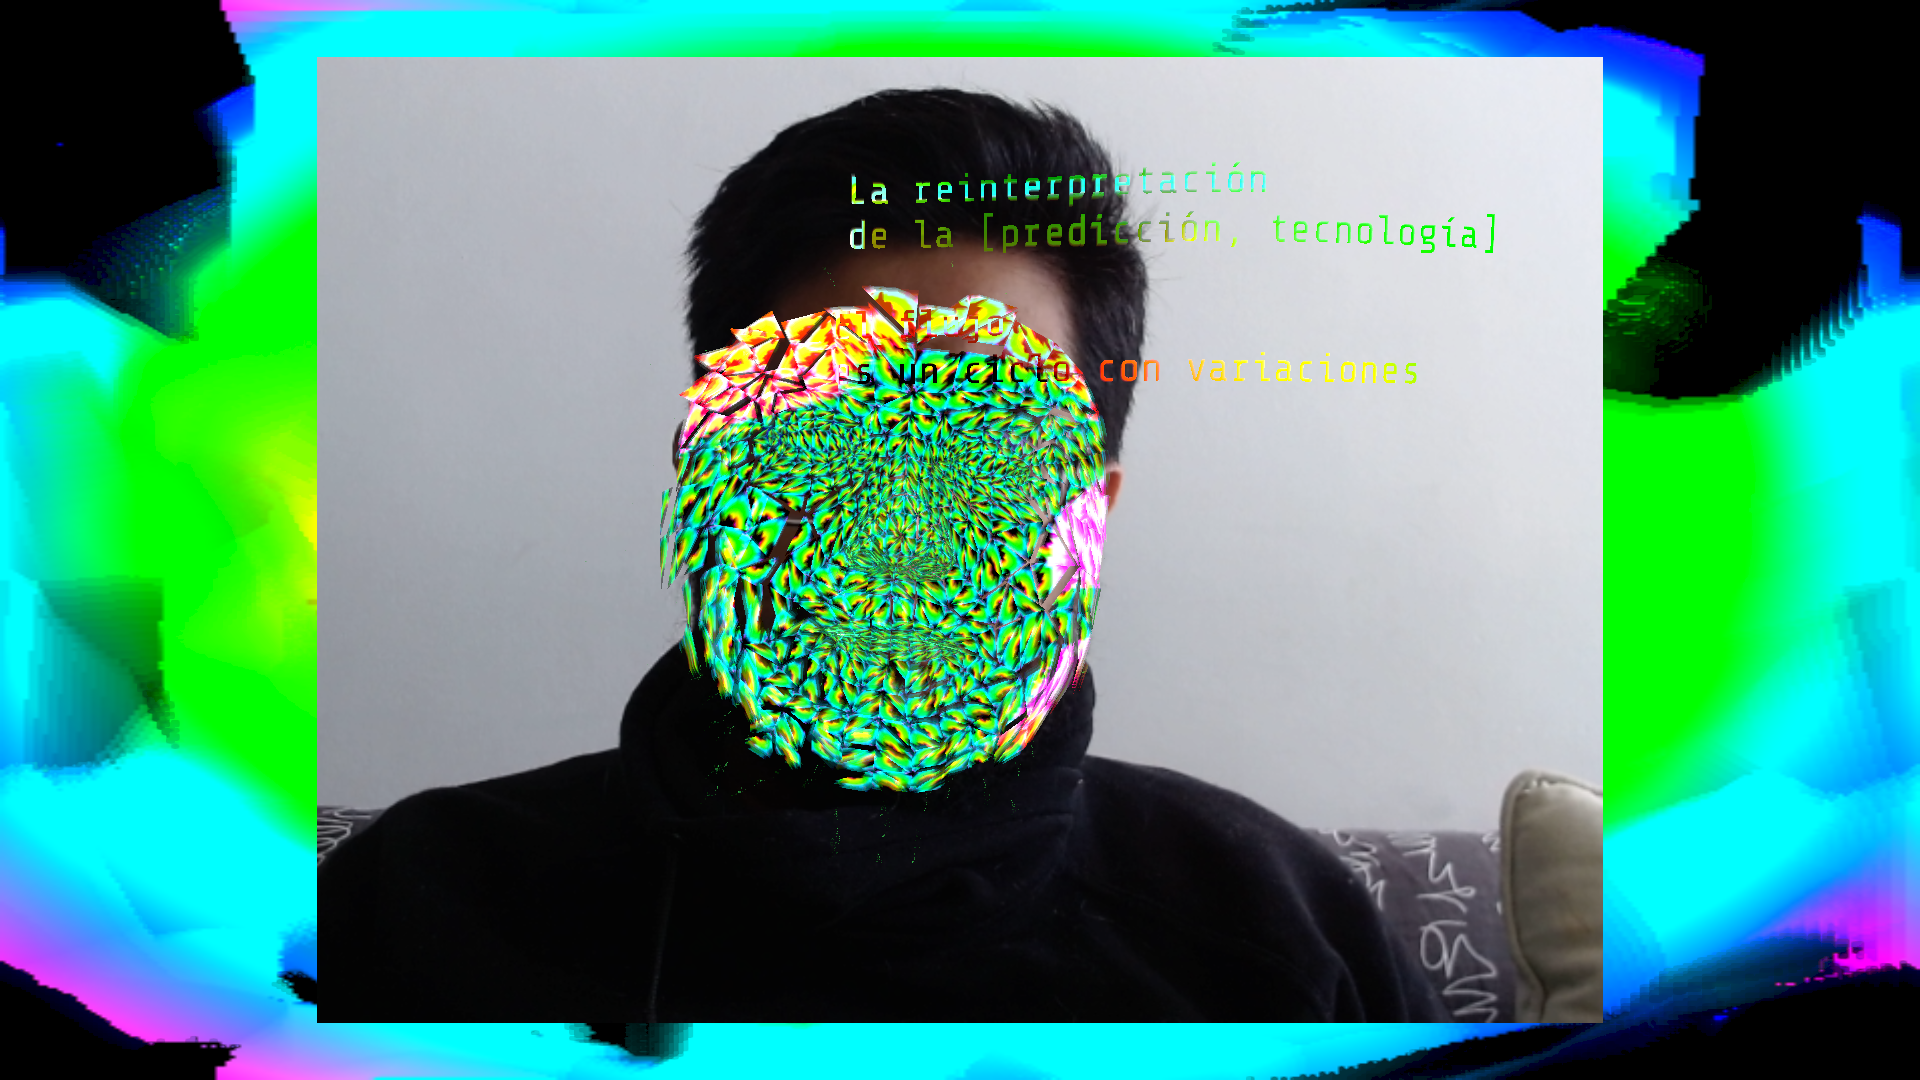
\includegraphics[width=\textwidth]{img/antiHydra2.png}
  \caption{Captura de Anti - Emilio Ocelotl}
  \label{fig:anti}
\end{figure}
El proceso de escritura e investigación presente en \textit{Panorama} permitió enlazar la documentación, propia y externa, con la perspectiva de investigación. Consideramos que la investigación artística y la metáfora como estrategias posibles para conceptos que atraviesan lo estético, lo tecnológico y lo investigativo. Proyectos de investigación, creación y escritura de software futuros podrían tener en cuenta el uso de conceptos transversales. 

Estas perspectivas pueden extenderse hacia una postura para la investigación de tecnología y el papel que juegan en la política de los espacios físicos y virtuales, como el cuarto propio \citep{cuartopropio} o el buen conocer \citep{plato}. Podríamos relacionar estos procesos con el giro de los nuevos medios descrito por \cite{manovichlanguage}, las implicaciones sociales de este giro y sobre todo, las consecuencias estéticas que a partir de este se abren y desenvuelven en la interpretación musical por medio de la computadora y otras prácticas afines. 

Destacamos el giro de los nuevos medios como un cambio de paradigma que la tecnología musical debe considerar por las implicaciones de los usos/críticas de las tecnologías de la información, las tendencias para la resolución de problemas relacionados con gestión de datos y las consecuencias estéticas que a veces se empalman y otras rebasan a la música y las perspectivas de investigación asociadas a esta disciplina. El rodeo o la realización de un motivo tecnológico como una perspectiva de investigación que pueda aportar en el aspecto tecnológico y teórico-metodológico y la investigación que implica música y expresiones audiovisuales con tecnología.

%\color{Fuchsia}

A manera de cierre, consideramos que la observación podría enlazarse con manifiestos, posturas políticas y alternativas en la organización que dialogan con la escritura de software como desarrollo tecnológico y como acto creativo. Tal es el caso de la práctica de \textit{live coding} y la transparencia de los procesos o el uso de interfaces de texto \citep{collinsLivecoding}, el manifiesto de una servidora feminista \citep{feministserver} o la arquitectura de distribución de información par a par, que persigue la distribución y la descentralización en redes que posibilitan espacios virtuales \citep{cyberspace} y que incluso puede extenderse al autocuidado y formas alternativas de expresar relaciones sociales en red \citep{dwc} o desmantelar y reconfigurar tecnologías en relación a la estética, a la tecnología y a la organización social distribuida. 



% Objetivo de la investigación: realización de sistemas ligeros que puedan ser accesibles con uan tecnología relativamente económica para la computadora para el navegador. Los eventos pudieron realizarse, sin dificultades, quedo pendiente la resolución de una versión para el navegador. 

% Objetivo secundario: documentación de software y del proceso 

% Agenda de enunaciación de trabajos y reflexiones para el futuro.

% Antes que nada, la perspectiva de observación / investigación. ¿Por qué esto tendría que estar al inicio? Diferencia entre documentación y observación 

% Documentación propia y ajena. 

% Software escrito en el contexto de trabajos y piezas post pandemia

% Aquí puede ir lo de THREE.studies y Anti 

% Reflexiones pendientes que pueden extenderse en otros momentos de investigación 

% Consecuencias no buscadas que se empalman con el proyecto. Idea interesante proveniente de Bruno Latour: es tiempo de girar de un paradigma que abierta o tácitamente refiere a la escala de recursos de la computadora. Si podemos trasladar esta lógica a una economía de los recursos de la computadora, no es tiempo ya de dar un giro que deje de hacer patente lo económico para dar paso a lo ecológico. 

%%%%%%%%%%%%%%%%% Pendiente: servidores, autogestión y cuerpós 

% Hacerse cargo de la gestión de los datos y de los servidores tiene que ver con los cuerpos, El cuerpo es infraestructura que posibilita el funcionamiento de los servidores.

% Servidores de todas formas generan consecuencias ecológicas > cambios significativos tendrían que ser de empresas y no tanto proyectos chiquitos. 

% Reducción de energía > responsabilidad de datos

% Cuerpo medio e interfaz como se articulan > Hans Belting > Imagen medium y cuerpo. Un nuevo acercamiento a la iconología > ¿Imágenes tradicionales? 

% PeerTube transitar del modo servidor a la forma de estructurar la experiencia en modo p2p
